% =====================================================================
%  Campus Marketplace -- UCS503 Software Engineering
%  Final project report in the TIET report template format
%  Compile with:  pdflatex campus_marketplace_report.tex  (run 3 times)
% =====================================================================
\documentclass[12pt,letterpaper,twoside,openany]{report}

\usepackage[T1]{fontenc}
\usepackage{lmodern}
\usepackage[utf8]{inputenc}
\usepackage[margin=1in,headheight=15pt]{geometry}
\usepackage{microtype}
\usepackage{amsmath}
\usepackage{booktabs}
\usepackage{float}
\usepackage{array}
\usepackage{tabularx}
\usepackage{enumitem}
\usepackage{xcolor}
\usepackage{graphicx}
\usepackage{titlesec}
\usepackage{fancyhdr}
\usepackage[skip=6pt]{caption}
\usepackage{tikz}
\usetikzlibrary{arrows.meta,positioning,shapes.geometric,shapes.multipart,calc,fit,backgrounds}
\usepackage{pgfplots}
\pgfplotsset{compat=1.16}
\usepackage[hidelinks]{hyperref}
\usepackage[hyperpageref]{backref}
\hypersetup{pdftitle={Campus Marketplace - UCS503 Software Engineering}}
\renewcommand*{\backref}[1]{}
\renewcommand*{\backrefalt}[4]{%
  \ifcase #1 \or (cit.\ on p.~#2).\else (cit.\ on pp.~#2).\fi}

\setlength{\parindent}{1.2em}
\renewcommand{\arraystretch}{1.12}
\newcolumntype{L}[1]{>{\raggedright\arraybackslash}p{#1}}

% ---------------------------------------------------------------- headings (TIET template style)
\titleformat{\chapter}[display]
  {\normalfont\raggedleft}
  {\large\bfseries\chaptertitlename\ \thechapter}
  {4pt}
  {\Huge}[\vspace{2pt}\titlerule]
\titleformat{name=\chapter,numberless}[display]
  {\normalfont\raggedleft}{}{0pt}{\Huge\bfseries}[\vspace{2pt}\titlerule]
\titlespacing*{\chapter}{0pt}{0pt}{36pt}
\titleformat{\section}{\normalfont\Large\bfseries}{\thesection}{1em}{}
\titleformat{\subsection}{\normalfont\large\bfseries}{\thesubsection}{1em}{}
\titlespacing*{\section}{0pt}{22pt}{12pt}
\titlespacing*{\subsection}{0pt}{16pt}{8pt}

% ---------------------------------------------------------------- header / footer
\newcommand{\course}{UCS503 - Software Engineering}
\pagestyle{fancy}
\fancyhf{}
\fancyhead[LE]{\small\thepage\quad\course}
\fancyhead[RO]{\small\course\quad\thepage}
\renewcommand{\headrulewidth}{0.4pt}
\fancypagestyle{plain}{\fancyhf{}\renewcommand{\headrulewidth}{0pt}}

\setlist[enumerate]{leftmargin=2.2em,itemsep=3pt}
\setlist[itemize]{leftmargin=2.2em,itemsep=3pt}

\newcommand{\code}[1]{\texttt{#1}}
\newcommand{\st}[1]{\textsc{#1}}

% ---------------------------------------------------------------- TikZ styles
\tikzset{
  >={Stealth[length=2.2mm]},
  box/.style={draw,rectangle,fill=white,align=center,font=\scriptsize,inner sep=3pt},
  gbox/.style={box,fill=gray!18},
  act/.style={draw,rectangle,rounded corners=2pt,fill=white,align=center,font=\scriptsize,
              text width=3.4cm,minimum height=0.75cm,inner sep=2pt},
  dec/.style={draw,diamond,aspect=2.1,fill=gray!18,align=center,font=\scriptsize,inner sep=1pt,
              text width=1.75cm},
  uc/.style={draw,ellipse,fill=white,align=center,font=\scriptsize,minimum width=3.4cm,
             minimum height=0.85cm,inner sep=1pt},
  guc/.style={uc,fill=gray!18},
  lbl/.style={font=\scriptsize\itshape,fill=white,inner sep=1pt},
  cls/.style={draw,rectangle split,rectangle split parts=3,rectangle split part fill={gray!18,white,white},
              font=\scriptsize,align=left,text width=4.75cm,inner sep=2.5pt},
}
\newcommand{\actor}[3]{% name, position, label
  \begin{scope}[shift={#2}]
    \draw (0,0.32) circle (0.13);
    \draw (0,0.19) -- (0,-0.22);
    \draw (-0.24,0.06) -- (0.24,0.06);
    \draw (0,-0.22) -- (-0.18,-0.55);
    \draw (0,-0.22) -- (0.18,-0.55);
    \node[font=\scriptsize,align=center,below] at (0,-0.58) {#3};
    \coordinate (#1) at (0,0);
  \end{scope}}


% =====================================================================
\begin{document}

% ---------------------------------------------------------------- title page
\begin{titlepage}
\centering
{\bfseries \course\par}
\vspace{2.4cm}
{\LARGE\bfseries Campus Marketplace\par}
\vspace{0.3cm}
{\small A Verified-Student Platform for Buying, Borrowing, Selling and Lending\\
with ML-Assisted Fair-Price Recommendation\par}
\vspace{2.2cm}
{\bfseries Submitted by:\par}
\vspace{0.3cm}
{\small
\texttt{1024031047} Shweta Agarwal\\
\texttt{1024031049} Shrasthi Singh Rathore\\
\texttt{1024031021} Raksha Pandey\par}
\vspace{0.4cm}
{\small Group: \texttt{3C73} BE Third Year, CSE\par}
\vspace{2.2cm}
{\bfseries Submitted to:\par}
\vspace{0.3cm}
{\small Dr. Jhonsy Bansal\par}
\vfill
{\small End-Semester Evaluation\par}
\vspace{0.2cm}
{\bfseries Computer Science and Engineering Department\par}
\vspace{0.1cm}
{\small Thapar Institute of Engineering and Technology, Patiala\par}
\end{titlepage}

% ---------------------------------------------------------------- contents
\clearpage
\pagenumbering{arabic}
\setcounter{page}{2}
\tableofcontents

% =====================================================================
\chapter{Introduction}

\section{Background and Context}
A university campus is a small, dense economy. Every semester, first-year students buy the same
textbooks, drafters and lab coats that graduating students are about to discard; hostel residents
need kettles, mattresses and cycles for a few months only; and short-term needs such as a
scientific calculator for one examination are better served by borrowing than by purchasing. Today
this exchange happens through scattered group chats and notice boards, which are unsearchable,
unstructured and unaccountable.

Public classified websites do not solve the problem. They are open to anyone, so a buyer cannot
tell whether the seller is a genuine fellow student; they provide no guidance on what a used item
is worth; and they have no notion of lending, where an item changes hands for a limited period
and must be returned. Campus Marketplace is a web application that closes these gaps for a single
campus community. It is built as a React single-page application, an Express.js REST API backed by
MongoDB, and a separate Python FastAPI service that hosts a fair-price recommendation model, and
it gave the team the opportunity to apply the full software engineering life cycle (requirements,
design, implementation and evaluation) to a multi-tier, data-driven system.

\subsection{Problem Statement}
Design and implement a web platform in which only verified members of a campus can list items
for sale or for lending, discover items nearby, communicate with each other, complete purchases or
loans with an auditable transaction history, and build a measurable reputation, while the system
itself assists sellers with a fair, explainable price and keeps every payment consistent and
verifiable. The system targets a single campus whose allowed e-mail domains are configured by the
administrator; physical hand-over of items happens on campus and is arranged, not performed, by the
system.

\section{Project Objectives}
\begin{enumerate}
  \item \textbf{Objective 1 -- Verified access:} restrict every marketplace endpoint to users whose
        college e-mail identity has been verified by OTP or Google Sign-In, and reject all other
        sessions, as checked by automated API tests.
  \item \textbf{Objective 2 -- Complete trading workflow:} support the four intents buy, borrow, sell and
        lend, including a loan life cycle with due dates, extensions, overdue detection and return
        confirmation.
  \item \textbf{Objective 3 -- ML-assisted pricing:} give every seller a suggested price and a fair-price
        band from a trained model whose test error is clearly below a naive baseline, with a labelled
        formula fallback and the final price always remaining the seller's decision.
  \item \textbf{Objective 4 -- Secure and consistent checkout:} take the price from the database, reserve
        an item while one buyer pays, verify every payment signature on the server, and refund payments
        that arrive after an item is no longer available.
  \item \textbf{Objective 5 -- Trust and privacy:} compute a trust score for each user, never expose exact
        coordinates, and accept only validated photos uploaded by the listing owner.
  \item \textbf{Objective 6 -- Maintainable architecture:} separate the user interface, the business API
        and the ML service so that each can be developed, tested and deployed independently, all within
        the semester's six development increments.
\end{enumerate}

These objectives are specific (each names one capability), measurable (each is verified by an
automated test or a reported metric in Chapter~\ref{ch:results}), achievable with the chosen stack,
relevant to a campus community, and were time-bound to the semester plan shown in Figure~\ref{fig:sdlc}.

\section{Requirements}
The objectives were refined into the stakeholders, functional requirements and non-functional
requirements listed in Tables~\ref{tab:stake}--\ref{tab:nfr}; Table~\ref{tab:env} gives the development
and runtime environment.

\begin{table}[H]
\centering
\caption{Stakeholders and their interaction with the system.}\label{tab:stake}
\small
\begin{tabularx}{\textwidth}{@{}L{2.6cm}X@{}}
\toprule
\textbf{Role} & \textbf{Description}\\
\midrule
Student & A verified campus member. The same account can act as buyer, borrower, seller or
lender, so a single role covers all four intents.\\
Administrator & Reviews listings in the moderation queue, approves or rejects held listings, and
can refund a completed payment.\\
ML service & Internal system actor that returns fair-price recommendations to the API over HTTP.\\
Payment gateway & External actor (Razorpay, or a signed development gateway) that creates orders,
confirms payments, sends webhooks and processes refunds.\\
Identity provider & Google OAuth 2.0 and an SMTP server used for verification.\\
Image storage & Cloudinary, which stores and resizes listing photos (local disk in development).\\
\bottomrule
\end{tabularx}
\end{table}

\begin{table}[H]
\centering
\caption{Functional requirements.}\label{tab:fr}
\small
\begin{tabularx}{\textwidth}{@{}L{1.0cm}X@{}}
\toprule
\textbf{ID} & \textbf{Requirement}\\
\midrule
FR1 & A user shall register with a college e-mail, verify it with a one-time password, and log in; Gmail and
allowed Google accounts shall use Google Sign-In.\\
FR2 & The system shall reject any marketplace request from an unverified user, and any administrator
request from a non-administrator.\\
FR3 & A student shall create, edit, view and remove listings for sale or lending, with category, condition,
brand, age, original price, description and up to six photos.\\
FR4 & The system shall return a fair-price band, a recommended price, a confidence value, an explanation
and the source of the estimate (ML model or formula), and shall show the prices of similar campus
listings when at least four exist.\\
FR5 & Photos shall be uploaded when selected, checked for a real image type and size limit, stored in cloud
storage, and referenced by URL; a listing may only use photos uploaded by its own seller.\\
FR6 & A student shall search and filter listings and keep a watchlist.\\
FR7 & A student shall chat with a listing owner through stored messages.\\
FR8 & A student shall request to borrow an item; the lender shall approve or reject, set or change the due
date, and approve extensions.\\
FR9 & The system shall track loan status (requested, active, due soon, overdue, return requested,
completed) and notify users.\\
FR10 & A purchase shall be charged at the price stored on the listing, the item shall be reserved during
checkout, and the sale shall be marked paid only after the payment signature or a signed webhook has
been verified on the server.\\
FR11 & Buyers and sellers shall be able to opt in to nearby discovery separately; exact coordinates shall
never be returned by any API.\\
FR12 & The system shall maintain a trust score from completed transactions, on-time returns, reviews and
upheld reports.\\
FR13 & An administrator shall view the moderation queue, approve or reject held listings, and refund
payments.\\
FR14 & The system shall export real, verified sales so that the price model can be retrained on campus
data.\\
\bottomrule
\end{tabularx}
\end{table}

\begin{table}[H]
\centering
\caption{Non-functional requirements.}\label{tab:nfr}
\small
\begin{tabularx}{\textwidth}{@{}L{2.6cm}X@{}}
\toprule
\textbf{Attribute} & \textbf{Requirement}\\
\midrule
Security & Passwords hashed with bcrypt; OTPs stored only as salted hashes with expiry, attempt and
resend limits; stateless JWT sessions; rate limiting on authentication, OTP, upload and general
API traffic; constant-time comparison of payment signatures; uploaded files identified by their
content, never by the client's file name.\\
Privacy & Exact latitude and longitude are never exposed; listing positions are blurred by 80--220\,m,
only approximate distances are shown, and stored positions expire after seven days.\\
Consistency & An item can be reserved by only one buyer at a time; a payment is finalised exactly once
even when the browser callback and the webhook both arrive.\\
Availability & The API shall start without an installed MongoDB (in-memory fallback) and shall keep
accepting listings when the ML service is down, using a labelled formula estimate.\\
Maintainability & Three independently runnable components with environment-based configuration and a
documented REST interface.\\
Usability & Responsive interface; clear labels for development-mode payments, local photo storage and
AI estimates that are not guaranteed market values.\\
Testability & Automated API tests for authentication, listings, uploads, location, loans, payments and
pricing, and automated sanity tests for the price model.\\
\bottomrule
\end{tabularx}
\end{table}

\begin{table}[H]
\centering
\caption{Development and runtime environment.}\label{tab:env}
\small
\begin{tabularx}{\textwidth}{@{}L{2.0cm}X@{}}
\toprule
\textbf{Item} & \textbf{Requirement}\\
\midrule
Client & Any modern browser with JavaScript; Geolocation API for optional nearby discovery.\\
Server & Node.js runtime with npm; MongoDB (local, Atlas, or the bundled in-memory server); Python 3
for the ML service.\\
Libraries & React, React Router, Tailwind CSS, Vite; Express, Mongoose, jsonwebtoken, bcryptjs, multer,
nodemailer, Razorpay SDK, Cloudinary SDK, Google Auth Library; FastAPI, scikit-learn, pandas,
NumPy, joblib.\\
Services & Optional Razorpay test keys, Cloudinary account, SMTP server and Google OAuth client.\\
Hardware & A commodity laptop is sufficient for development, model training and demonstration.\\
\bottomrule
\end{tabularx}
\end{table}

% =====================================================================
\chapter{Methodology and Design}\label{ch:design}

\section{System Architecture}
The project followed an iterative and incremental life cycle~\cite{larman}. The work was divided into
six increments, and each increment was taken through the same five phases (requirements, design,
implementation, testing, and integration review); the feedback from each review fed directly into the
requirements of the next increment. Figure~\ref{fig:sdlc} shows the cycle and the increments delivered.
This model suited the project because the user interface existed first as a prototype on mock data,
and the backend, identity, marketplace logic, machine-learning and hardening work were added in
successive, independently testable steps. The last increment was itself driven by review feedback:
the first price model generalised poorly, and the first image and payment designs did not survive
realistic use. All diagrams in this report are drawn natively in TikZ in a monochrome palette.

\begin{figure}[h]
\centering
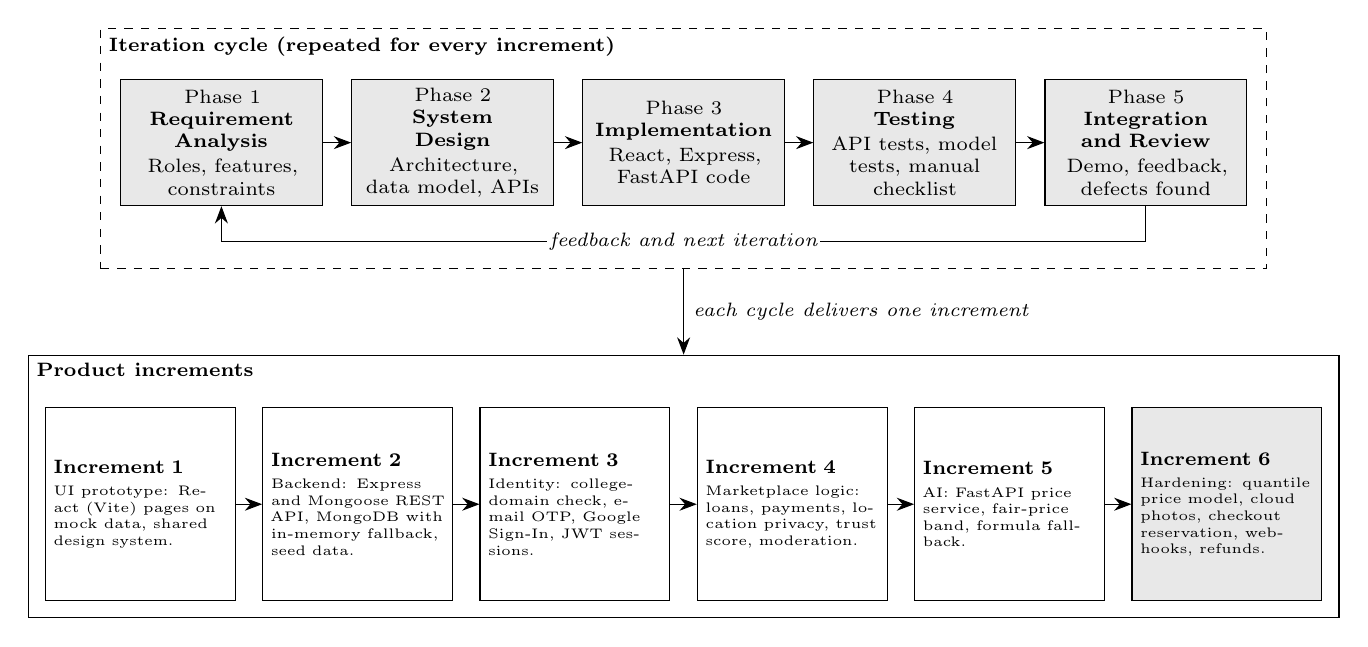
\begin{tikzpicture}[
  ph/.style={box,fill=gray!18,text width=2.35cm,minimum height=1.6cm},
  inc/.style={box,text width=2.2cm,minimum height=2.45cm,align=left,anchor=north,
              font=\tiny},
  node distance=0.36cm]
  % phases
  \node[ph] (p1) {Phase 1\\\textbf{Requirement}\\\textbf{Analysis}\\[1pt]Roles, features,\\constraints};
  \node[ph,right=of p1] (p2) {Phase 2\\\textbf{System}\\\textbf{Design}\\[1pt]Architecture,\\data model, APIs};
  \node[ph,right=of p2] (p3) {Phase 3\\\textbf{Implementation}\\[1pt]React, Express,\\FastAPI code};
  \node[ph,right=of p3] (p4) {Phase 4\\\textbf{Testing}\\[1pt]API tests, model\\tests, manual\\checklist};
  \node[ph,right=of p4] (p5) {Phase 5\\\textbf{Integration}\\\textbf{and Review}\\[1pt]Demo, feedback,\\defects found};
  \foreach \a/\b in {p1/p2,p2/p3,p3/p4,p4/p5} \draw[->] (\a) -- (\b);
  \draw[->] (p5.south) -- ++(0,-0.45) -| node[pos=0.25,lbl,fill=white]{feedback and next iteration} (p1.south);
  \begin{scope}[on background layer]
    \node[draw,dashed,inner sep=7pt,fit={(p1)(p5)($(p1.south)+(0,-0.55)$)($(p1.north)+(0,0.4)$)}] (cyc) {};
  \end{scope}
  \node[font=\scriptsize\bfseries,anchor=north west,inner sep=3pt] at (cyc.north west) {Iteration cycle (repeated for every increment)};
  % increments
  \path (cyc.south) ++(0,-1.75) coordinate (itop);
  \node[inc] (i1) at ($(itop)+(-6.90,0)$) {\textbf{\scriptsize Increment 1}\\[2pt]UI prototype: React (Vite) pages on mock data, shared design system.};
  \node[inc] (i2) at ($(itop)+(-4.14,0)$) {\textbf{\scriptsize Increment 2}\\[2pt]Backend: Express and Mongoose REST API, MongoDB with in-memory fallback, seed data.};
  \node[inc] (i3) at ($(itop)+(-1.38,0)$) {\textbf{\scriptsize Increment 3}\\[2pt]Identity: college-domain check, e-mail OTP, Google Sign-In, JWT sessions.};
  \node[inc] (i4) at ($(itop)+(1.38,0)$) {\textbf{\scriptsize Increment 4}\\[2pt]Marketplace logic: loans, payments, location privacy, trust score, moderation.};
  \node[inc] (i5) at ($(itop)+(4.14,0)$) {\textbf{\scriptsize Increment 5}\\[2pt]AI: FastAPI price service, fair-price band, formula fallback.};
  \node[inc,fill=gray!18] (i6) at ($(itop)+(6.90,0)$) {\textbf{\scriptsize Increment 6}\\[2pt]Hardening: quantile price model, cloud photos, checkout reservation, webhooks, refunds.};
  \foreach \a/\b in {i1/i2,i2/i3,i3/i4,i4/i5,i5/i6} \draw[->] (\a) -- (\b);
  \begin{scope}[on background layer]
    \node[draw,inner sep=6pt,fit={(i1)(i6)($(i1.north)+(0,0.45)$)}] (incs) {};
  \end{scope}
  \node[font=\scriptsize\bfseries,anchor=north west,inner sep=3pt] at (incs.north west) {Product increments};
  \draw[->] (cyc.south) -- node[right,font=\scriptsize\itshape]{each cycle delivers one increment} (incs.north);
\end{tikzpicture}
\caption{SDLC diagram: iterative and incremental model used for Campus Marketplace.}\label{fig:sdlc}
\end{figure}

\subsection{High-Level Design}
The system is organised as three independently runnable tiers: a React single-page application that
talks only to the REST API through a central client module, an Express.js API that applies CORS, rate
limiting and JWT authentication before requests reach the route modules and business
services~\cite{fielding}, and a separate FastAPI service that hosts the price model. Persistent data lives
in MongoDB, and identity, payment and image-storage providers are external services. Keeping the ML stack
in its own service means it can be trained, replaced or restarted without touching the API, and the API
degrades gracefully to a formula estimate when that service is unreachable. The design is described by
four UML models~\cite{uml}.

\paragraph{Use case model.} Figure~\ref{fig:usecase} shows the use cases inside the system boundary. A
single Student actor covers buyer, borrower, seller and lender because the same account performs all four
roles. The administrator works the moderation queue and can refund payments; the ML service and the
payment gateway are secondary actors that the system calls. Fair-price prediction \emph{extends} listing
creation, and making a payment \emph{includes} reserving the item and verifying the payment signature.

\begin{figure}[h]
\centering
\begin{tikzpicture}
  \draw (0,0) rectangle (9.8,-11.75);
  \node[font=\scriptsize\bfseries] at (4.9,-0.3) {Campus Marketplace System};
  % student use cases
  \node[uc] (u1) at (2.5,-1.3)  {Register and Verify\\College E-mail\\(OTP / Google)};
  \node[uc] (u2) at (2.5,-2.45)  {Browse, Search and\\Nearby Filter};
  \node[uc] (u3) at (2.5,-3.5)  {Manage Watchlist\\and Notifications};
  \node[uc] (u4) at (2.5,-4.55)  {Upload Listing\\Photos};
  \node[uc] (u5) at (2.5,-5.6)  {Create Listing\\(Sell / Lend)};
  \node[uc] (u6) at (2.5,-6.65)  {Chat with\\Listing Owner};
  \node[uc] (u7) at (2.5,-7.7)  {Request to\\Borrow};
  \node[uc] (u8) at (2.5,-8.75)  {Buy Item\\(Make Payment)};
  \node[uc] (u9) at (2.5,-9.8)  {Approve, Extend\\and Return Loans};
  \node[uc] (u10) at (2.5,-11.0) {Review and Rate Users};
  % right column
  \node[guc] (a1) at (7.4,-1.25) {Review Moderation\\Queue};
  \node[guc] (a2) at (7.4,-2.45) {Approve / Reject\\Held Listing};
  \node[guc] (a3) at (7.4,-3.6) {Refund Payment};
  \node[guc] (m1) at (7.4,-5.6) {Predict Fair\\Price Range};
  \node[guc] (r1) at (7.4,-8.0) {Reserve Item\\for Checkout};
  \node[guc] (v1) at (7.4,-9.5) {Verify Payment\\Signature};
  % actors
  \actor{stu}{(-1.5,-6.1)}{Student}
  \actor{adm}{(11.4,-2.4)}{Administrator}
  \actor{ml}{(11.4,-5.6)}{ML service\\(FastAPI)}
  \actor{pg}{(11.4,-9.5)}{Payment\\Gateway\\(Razorpay)}
  \foreach \u in {u1,u2,u3,u4,u5,u6,u7,u8,u9,u10} \draw (stu) -- (\u.west);
  \foreach \u in {a1,a2,a3} \draw (adm) -- (\u.east);
  \draw (ml) -- (m1.east);
  \draw (pg) -- (v1.east);
  \draw[dashed,->] (m1.west) -- node[lbl,above,sloped]{\guillemotleft extends\guillemotright} (u5.east);
  \draw[dashed,->] (u8.east) -- node[lbl,above,sloped,pos=0.55]{\guillemotleft includes\guillemotright} (r1.west);
  \draw[dashed,->] (u8.east) -- node[lbl,below,sloped,pos=0.55]{\guillemotleft includes\guillemotright} (v1.west);
\end{tikzpicture}
\caption{Use case diagram of Campus Marketplace.}\label{fig:usecase}
\end{figure}

\paragraph{Sequence model.} Figure~\ref{fig:seq} shows how the tiers interact when a seller prices and
publishes a listing. While the seller fills in the form, the interface asks the API for an estimate; the
API obtains the fair-price band from the ML service and the asking prices of similar listings from
MongoDB, and the interface shows both. When the seller confirms an asking price and publishes, the API
requests the recommendation again, stores it on the new listing, and returns the created listing.

\begin{figure}[h]
\centering
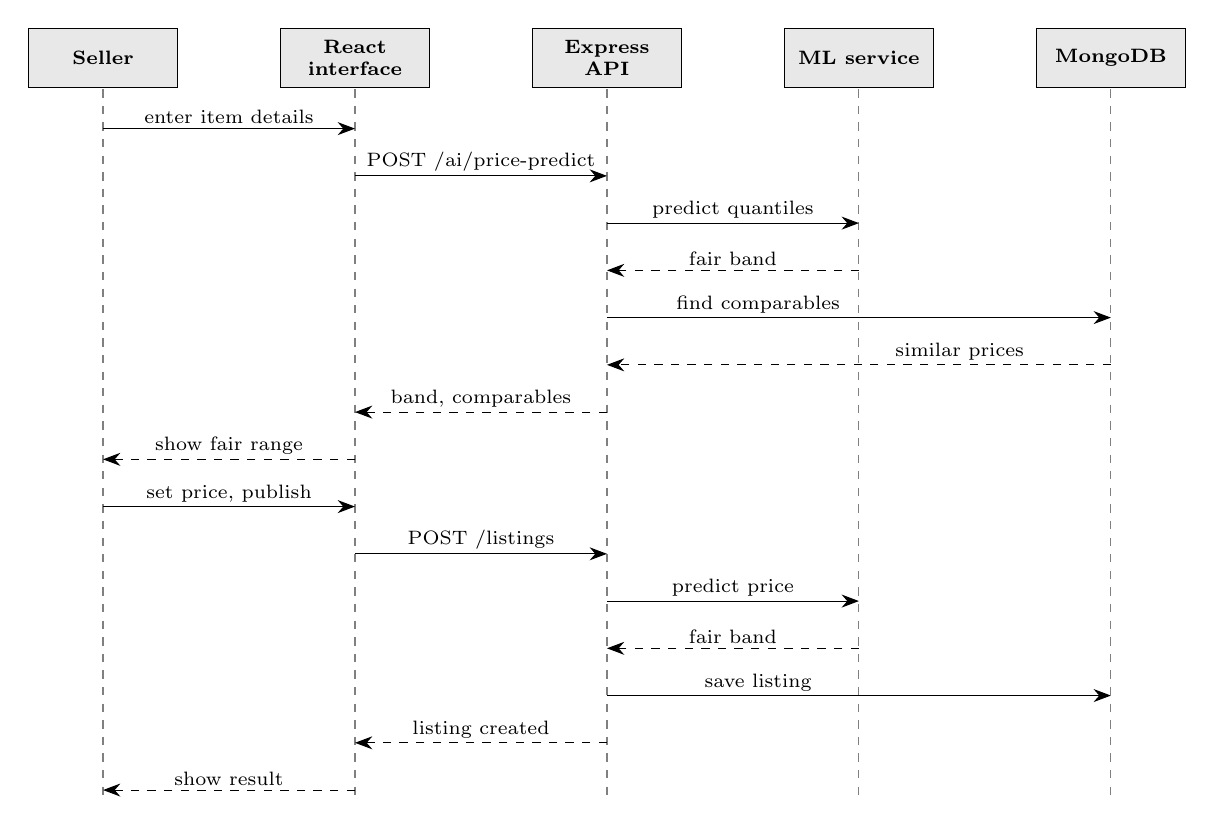
\begin{tikzpicture}[
  ll/.style={gbox,font=\scriptsize\bfseries,minimum width=1.9cm,minimum height=0.75cm},
  msg/.style={->},
  ret/.style={->,dashed},
  mt/.style={font=\scriptsize,above,inner sep=1.5pt}]
  \def\xs{0}\def\xr{3.2}\def\xa{6.4}\def\xm{9.6}\def\xd{12.8}
  \node[ll] at (\xs,0) {Seller};
  \node[ll] at (\xr,0) {React\\interface};
  \node[ll] at (\xa,0) {Express\\API};
  \node[ll] at (\xm,0) {ML service};
  \node[ll] at (\xd,0) {MongoDB};
  \foreach \x in {\xs,\xr,\xa,\xm,\xd} \draw[dashed,gray] (\x,-0.4) -- (\x,-9.4);
  \def\d{0.6}
  \draw[msg] (\xs,-1*\d-0.3) -- node[mt]{enter item details} (\xr,-1*\d-0.3);
  \draw[msg] (\xr,-2*\d-0.3) -- node[mt]{POST /ai/price-predict} (\xa,-2*\d-0.3);
  \draw[msg] (\xa,-3*\d-0.3) -- node[mt]{predict quantiles} (\xm,-3*\d-0.3);
  \draw[ret] (\xm,-4*\d-0.3) -- node[mt]{fair band} (\xa,-4*\d-0.3);
  \draw[msg] (\xa,-5*\d-0.3) -- node[mt,pos=0.3]{find comparables} (\xd,-5*\d-0.3);
  \draw[ret] (\xd,-6*\d-0.3) -- node[mt,pos=0.3]{similar prices} (\xa,-6*\d-0.3);
  \draw[ret] (\xa,-7*\d-0.3) -- node[mt]{band, comparables} (\xr,-7*\d-0.3);
  \draw[ret] (\xr,-8*\d-0.3) -- node[mt]{show fair range} (\xs,-8*\d-0.3);
  \draw[msg] (\xs,-9*\d-0.3) -- node[mt]{set price, publish} (\xr,-9*\d-0.3);
  \draw[msg] (\xr,-10*\d-0.3) -- node[mt]{POST /listings} (\xa,-10*\d-0.3);
  \draw[msg] (\xa,-11*\d-0.3) -- node[mt]{predict price} (\xm,-11*\d-0.3);
  \draw[ret] (\xm,-12*\d-0.3) -- node[mt]{fair band} (\xa,-12*\d-0.3);
  \draw[msg] (\xa,-13*\d-0.3) -- node[mt,pos=0.3]{save listing} (\xd,-13*\d-0.3);
  \draw[ret] (\xa,-14*\d-0.3) -- node[mt]{listing created} (\xr,-14*\d-0.3);
  \draw[ret] (\xr,-15*\d-0.3) -- node[mt]{show result} (\xs,-15*\d-0.3);
\end{tikzpicture}
\caption{Sequence diagram: price recommendation and publishing a listing.}\label{fig:seq}
\end{figure}

\paragraph{Activity model.} Figure~\ref{fig:activity} traces the end-to-end flow from sign-in to a
completed transaction. A user first proves a verified college identity. A seller uploads photos, enters
listing details and receives a fair-price band (or a labelled formula estimate if the ML service is
unreachable); after the seller fixes an asking price the listing becomes active. A sale reserves the item
and creates a payment order: an invalid signature releases the reservation, a payment that arrives after
the item was sold to someone else is refunded, and a valid payment marks the item sold. A loan proceeds
through the lender's approval, agreement on a meeting point and due date, and ends with a
lender-confirmed return.

\paragraph{Class model.} Figure~\ref{fig:class} shows the principal persistent classes. Each class maps to
a Mongoose schema and a MongoDB collection; attribute lists are abbreviated to the fields central to the
design. User is the hub: it owns listings, takes part in transactions, sends and receives messages, and
receives reviews. A Listing references the photos recorded in Upload, is the subject of transactions, and
may be placed in the Moderation queue. A Transaction may be settled by one Payment.

\begin{figure}[p]
\centering
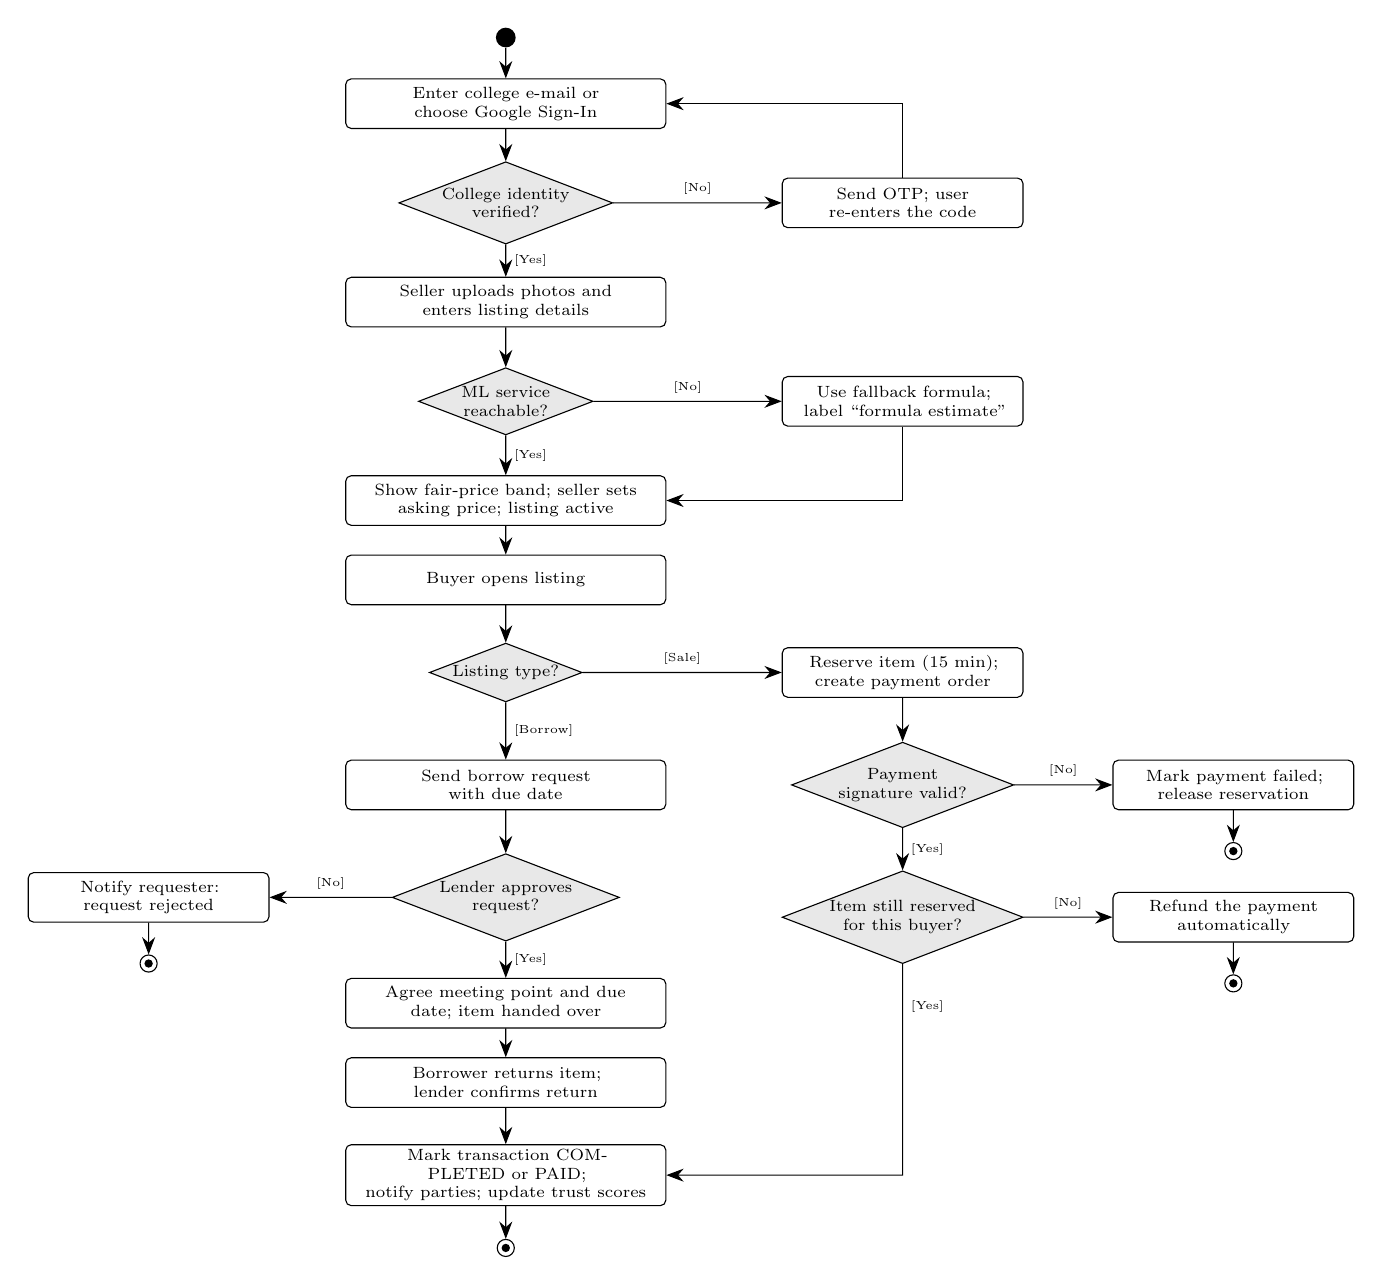
\begin{tikzpicture}[scale=0.84,transform shape,
  act/.style={draw,rectangle,rounded corners=2pt,fill=white,align=center,font=\scriptsize,
              text width=4.7cm,minimum height=0.75cm,inner sep=2pt},
  sact/.style={act,text width=3.5cm},
  dec/.style={draw,diamond,aspect=2.6,fill=gray!18,align=center,font=\scriptsize,inner sep=0.5pt},
  fin/.style={circle,draw,inner sep=2.6pt,path picture={\fill (path picture bounding box.center) circle (1.8pt);}},
  g/.style={font=\tiny}]
  \node[circle,fill=black,inner sep=3pt] (st) at (0,0) {};
  \node[act] (a1) at (0,-1.0) {Enter college e-mail or\\choose Google Sign-In};
  \node[dec] (d1) at (0,-2.5) {College identity\\verified?};
  \node[sact] (b1) at (6.0,-2.5) {Send OTP; user\\re-enters the code};
  \node[act] (a2) at (0,-4.0) {Seller uploads photos and\\enters listing details};
  \node[dec] (d2) at (0,-5.5) {ML service\\reachable?};
  \node[sact] (b2) at (6.0,-5.5) {Use fallback formula;\\label ``formula estimate''};
  \node[act] (a3) at (0,-7.0) {Show fair-price band; seller sets\\asking price; listing active};
  \node[act] (a4) at (0,-8.2) {Buyer opens listing};
  \node[dec] (d3) at (0,-9.6) {Listing type?};
  % sale branch
  \node[sact] (s1) at (6.0,-9.6) {Reserve item (15 min);\\create payment order};
  \node[dec] (d4) at (6.0,-11.3) {Payment\\signature valid?};
  \node[sact] (s2) at (11.0,-11.3) {Mark payment failed;\\release reservation};
  \node[fin] (e2) at (11.0,-12.3) {};
  \node[dec] (d5) at (6.0,-13.3) {Item still reserved\\for this buyer?};
  \node[sact] (s3) at (11.0,-13.3) {Refund the payment\\automatically};
  \node[fin] (e3) at (11.0,-14.3) {};
  % borrow branch
  \node[act] (l1) at (0,-11.3) {Send borrow request\\with due date};
  \node[dec] (d6) at (0,-13.0) {Lender approves\\request?};
  \node[sact] (l2) at (-5.4,-13.0) {Notify requester:\\request rejected};
  \node[fin] (e4) at (-5.4,-14.0) {};
  \node[act] (l3) at (0,-14.6) {Agree meeting point and due\\date; item handed over};
  \node[act] (l4) at (0,-15.8) {Borrower returns item;\\lender confirms return};
  \node[act] (fn) at (0,-17.2) {Mark transaction COMPLETED or PAID;\\notify parties; update trust scores};
  \node[fin] (e1) at (0,-18.3) {};
  % edges
  \draw[->] (st) -- (a1);
  \draw[->] (a1) -- (d1);
  \draw[->] (d1) -- node[above,g]{[No]} (b1);
  \draw[->] (b1.north) |- (a1.east);
  \draw[->] (d1) -- node[right,g]{[Yes]} (a2);
  \draw[->] (a2) -- (d2);
  \draw[->] (d2) -- node[above,g]{[No]} (b2);
  \draw[->] (b2.south) |- (a3.east);
  \draw[->] (d2) -- node[right,g]{[Yes]} (a3);
  \draw[->] (a3) -- (a4);
  \draw[->] (a4) -- (d3);
  \draw[->] (d3) -- node[above,g]{[Sale]} (s1);
  \draw[->] (s1) -- (d4);
  \draw[->] (d4) -- node[above,g]{[No]} (s2);
  \draw[->] (s2) -- (e2);
  \draw[->] (d4) -- node[right,g]{[Yes]} (d5);
  \draw[->] (d5) -- node[above,g]{[No]} (s3);
  \draw[->] (s3) -- (e3);
  \draw[->] (d5.south) -- node[right,g,pos=0.2]{[Yes]} (6.0,-17.2) -- (fn.east);
  \draw[->] (d3) -- node[right,g]{[Borrow]} (l1);
  \draw[->] (l1) -- (d6);
  \draw[->] (d6) -- node[above,g]{[No]} (l2);
  \draw[->] (l2) -- (e4);
  \draw[->] (d6) -- node[right,g]{[Yes]} (l3);
  \draw[->] (l3) -- (l4);
  \draw[->] (l4) -- (fn);
  \draw[->] (fn) -- (e1);
\end{tikzpicture}
\caption{Activity diagram: sign-in, listing, checkout and loan flow.}\label{fig:activity}
\end{figure}

\begin{figure}[p]
\centering
\resizebox{\textwidth}{!}{%
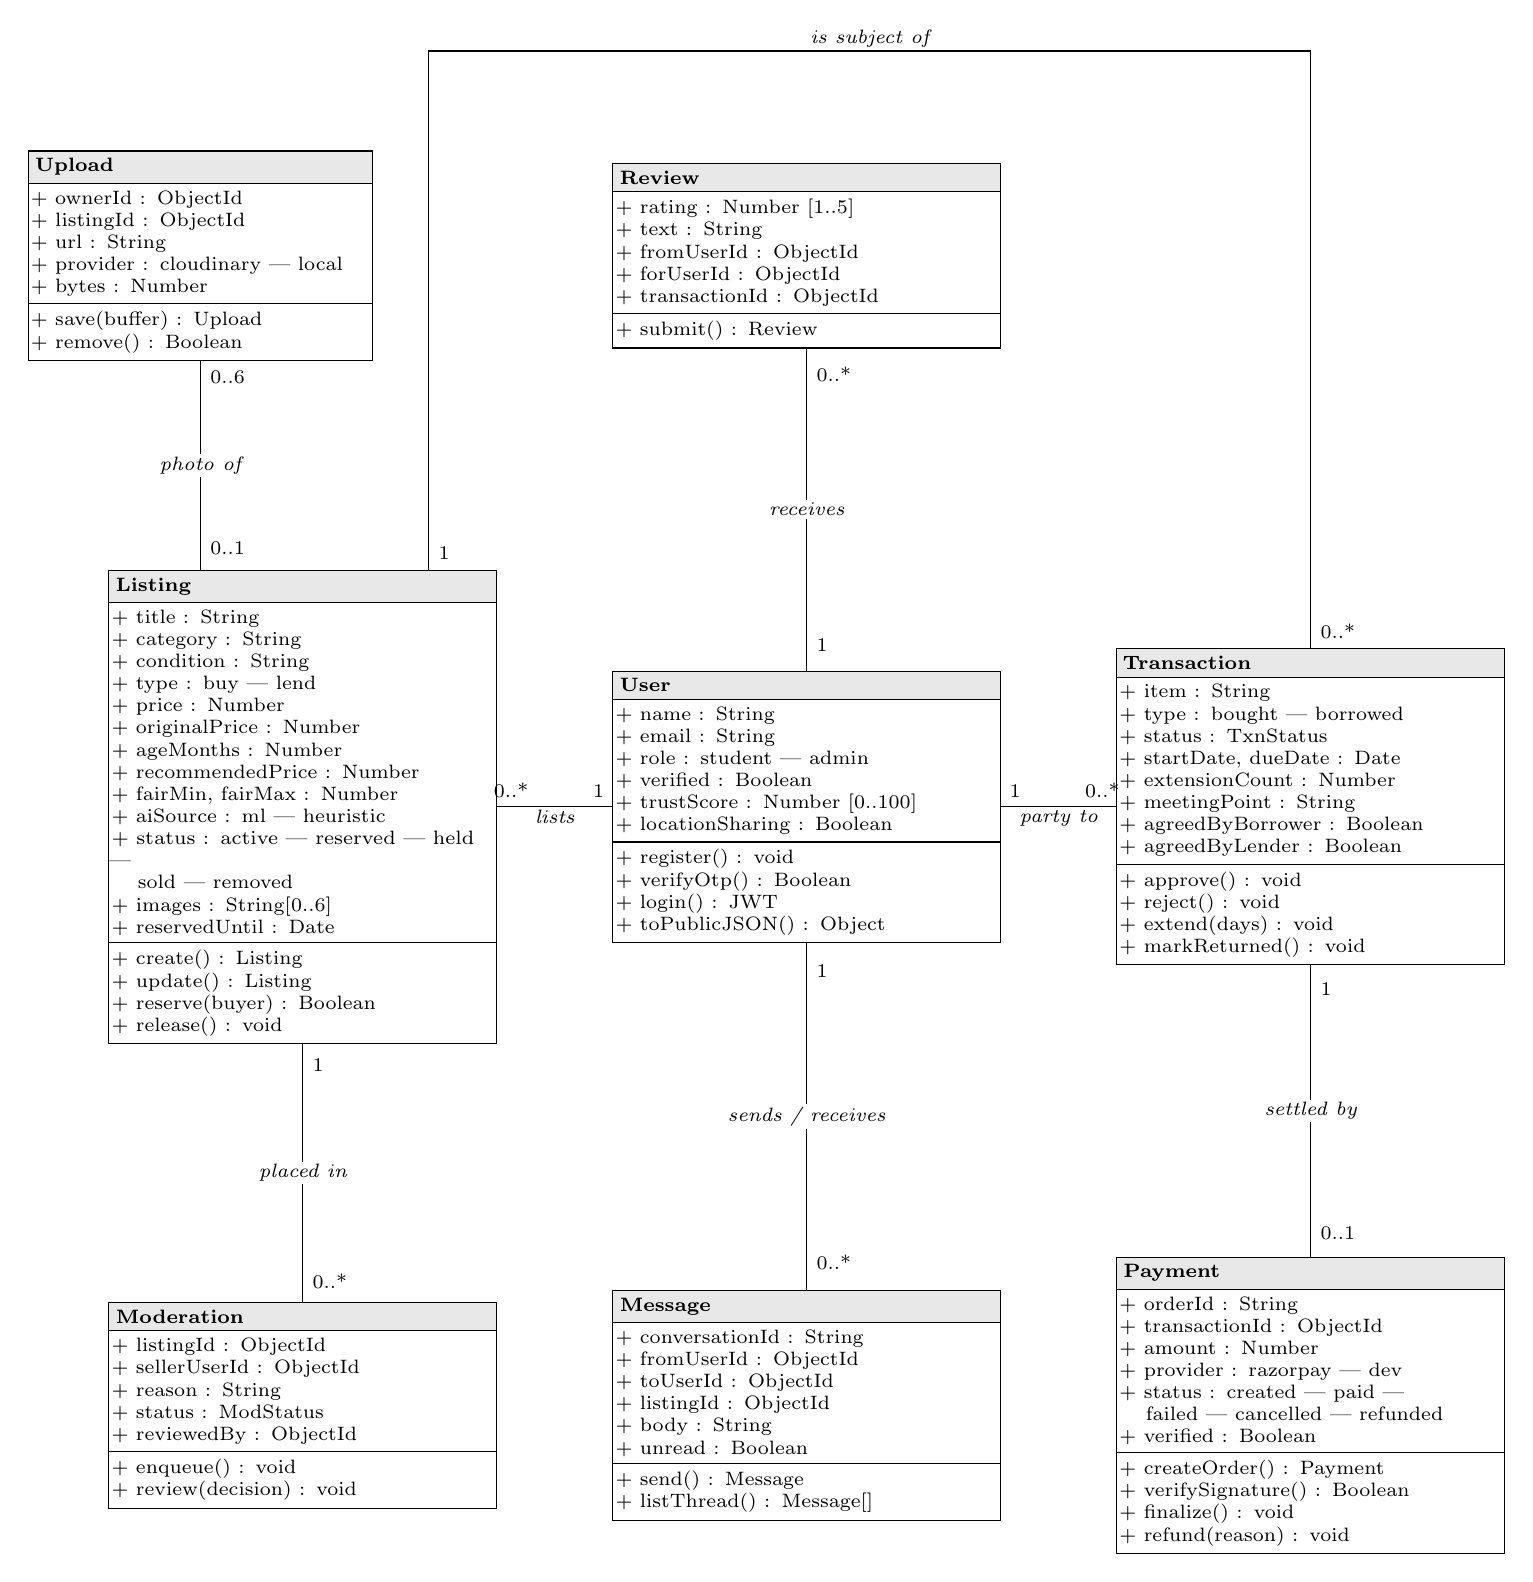
\begin{tikzpicture}
  % ---- middle row
  \node[cls] (lst) at (0,0) {\textbf{Listing}
    \nodepart{second}
    + title : String\\
    + category : String\\
    + condition : String\\
    + type : buy | lend\\
    + price : Number\\
    + originalPrice : Number\\
    + ageMonths : Number\\
    + recommendedPrice : Number\\
    + fairMin, fairMax : Number\\
    + aiSource : ml | heuristic\\
    + status : active | reserved | held |\\
    \quad sold | removed\\
    + images : String[0..6]\\
    + reservedUntil : Date
    \nodepart{third}
    + create() : Listing\\
    + update() : Listing\\
    + reserve(buyer) : Boolean\\
    + release() : void};
  \node[cls] (usr) at (6.4,0) {\textbf{User}
    \nodepart{second}
    + name : String\\
    + email : String\\
    + role : student | admin\\
    + verified : Boolean\\
    + trustScore : Number [0..100]\\
    + locationSharing : Boolean
    \nodepart{third}
    + register() : void\\
    + verifyOtp() : Boolean\\
    + login() : JWT\\
    + toPublicJSON() : Object};
  \node[cls] (txn) at (12.8,0) {\textbf{Transaction}
    \nodepart{second}
    + item : String\\
    + type : bought | borrowed\\
    + status : TxnStatus\\
    + startDate, dueDate : Date\\
    + extensionCount : Number\\
    + meetingPoint : String\\
    + agreedByBorrower : Boolean\\
    + agreedByLender : Boolean
    \nodepart{third}
    + approve() : void\\
    + reject() : void\\
    + extend(days) : void\\
    + markReturned() : void};
  % ---- top row
  \node[cls,text width=4.2cm] (upl) at (-1.3,7.0) {\textbf{Upload}
    \nodepart{second}
    + ownerId : ObjectId\\
    + listingId : ObjectId\\
    + url : String\\
    + provider : cloudinary | local\\
    + bytes : Number
    \nodepart{third}
    + save(buffer) : Upload\\
    + remove() : Boolean};
  \node[cls] (rev) at (6.4,7.0) {\textbf{Review}
    \nodepart{second}
    + rating : Number [1..5]\\
    + text : String\\
    + fromUserId : ObjectId\\
    + forUserId : ObjectId\\
    + transactionId : ObjectId
    \nodepart{third}
    + submit() : Review};
  % ---- bottom row
  \node[cls] (mod) at (0,-7.6) {\textbf{Moderation}
    \nodepart{second}
    + listingId : ObjectId\\
    + sellerUserId : ObjectId\\
    + reason : String\\
    + status : ModStatus\\
    + reviewedBy : ObjectId
    \nodepart{third}
    + enqueue() : void\\
    + review(decision) : void};
  \node[cls] (msg) at (6.4,-7.6) {\textbf{Message}
    \nodepart{second}
    + conversationId : String\\
    + fromUserId : ObjectId\\
    + toUserId : ObjectId\\
    + listingId : ObjectId\\
    + body : String\\
    + unread : Boolean
    \nodepart{third}
    + send() : Message\\
    + listThread() : Message[]};
  \node[cls] (pay) at (12.8,-7.6) {\textbf{Payment}
    \nodepart{second}
    + orderId : String\\
    + transactionId : ObjectId\\
    + amount : Number\\
    + provider : razorpay | dev\\
    + status : created | paid |\\
    \quad failed | cancelled | refunded\\
    + verified : Boolean
    \nodepart{third}
    + createOrder() : Payment\\
    + verifySignature() : Boolean\\
    + finalize() : void\\
    + refund(reason) : void};
  % ---- associations
  \draw (lst.east) -- node[above,font=\scriptsize,pos=0.12]{0..*} node[above,font=\scriptsize,pos=0.88]{1}
        node[below,lbl]{lists} (usr.west);
  \draw (usr.east) -- node[above,font=\scriptsize,pos=0.12]{1} node[above,font=\scriptsize,pos=0.88]{0..*}
        node[below,lbl]{party to} (txn.west);
  \draw (rev.south) -- node[right,font=\scriptsize,pos=0.08]{0..*} node[right,font=\scriptsize,pos=0.92]{1}
        node[lbl,midway]{receives} (usr.north);
  \draw (lst.south) -- node[right,font=\scriptsize,pos=0.08]{1} node[right,font=\scriptsize,pos=0.92]{0..*}
        node[lbl,midway]{placed in} (mod.north);
  \draw (usr.south) -- node[right,font=\scriptsize,pos=0.08]{1} node[right,font=\scriptsize,pos=0.92]{0..*}
        node[lbl,midway]{sends / receives} (msg.north);
  \draw (txn.south) -- node[right,font=\scriptsize,pos=0.08]{1} node[right,font=\scriptsize,pos=0.92]{0..1}
        node[lbl,midway]{settled by} (pay.north);
  \draw (upl.south) -- node[right,font=\scriptsize,pos=0.08]{0..6} node[right,font=\scriptsize,pos=0.9]{0..1}
        node[lbl,midway]{photo of} (upl.south |- lst.north);
  \draw ($(lst.north)+(1.6,0)$) node[above right,font=\scriptsize]{1} -- (1.6,9.6)
        -- node[lbl,above]{is subject of} (12.8,9.6) -- (txn.north) node[above right,font=\scriptsize]{0..*};
\end{tikzpicture}}
\caption{Class diagram of the persistent domain model.}\label{fig:class}
\end{figure}

\subsection{Technical Stack}
\begin{itemize}
  \item \textbf{Framework/Language:} JavaScript with React 19, React Router 7 and Vite on the
        client~\cite{react}; Node.js with Express 4 on the server~\cite{express}; Python with
        FastAPI~\cite{fastapi} for the ML service.
  \item \textbf{Database:} MongoDB~\cite{mongodb} accessed through Mongoose, with an automatic fallback to
        an in-memory MongoDB server for development.
  \item \textbf{Tools:} npm and pip, oxlint, the Node test runner, Python \code{unittest}, Git and GitHub,
        Overleaf for this report.
  \item \textbf{Libraries:} Tailwind CSS, jsonwebtoken, bcryptjs, express-rate-limit, multer, nodemailer,
        Google Auth Library, the Razorpay and Cloudinary SDKs; scikit-learn~\cite{sklearn}, pandas, NumPy
        and joblib.
\end{itemize}
Table~\ref{tab:stack} maps each technology to its layer and purpose.

\begin{table}[htbp]
\centering
\caption{Technology stack by layer.}\label{tab:stack}
\small
\begin{tabularx}{\textwidth}{@{}L{2.0cm}L{5.0cm}X@{}}
\toprule
\textbf{Layer} & \textbf{Technology} & \textbf{Purpose}\\
\midrule
Frontend & React 19, React Router 7, Vite, Tailwind CSS~\cite{react} & Single-page UI, protected routes, filters, favourites, dashboards.\\
API & Node.js, Express 4~\cite{express}, Mongoose & REST endpoints, validation, business rules.\\
Database & MongoDB~\cite{mongodb} & Persistence for users, listings, loans, messages, payments, uploads and reviews.\\
Security & jsonwebtoken, bcryptjs, express-rate-limit & Sessions~\cite{jwt}, password hashing, throttling.\\
Identity & Google Auth Library, nodemailer & OAuth 2.0 sign-in~\cite{oauth} and OTP e-mail.\\
Payments & Razorpay SDK, HMAC-SHA256~\cite{hmac} & Order creation, signature and webhook verification, refunds.\\
Storage & multer, Cloudinary SDK~\cite{cloudinary} & Photo upload, resizing and CDN delivery; local disk in development.\\
ML service & Python, FastAPI~\cite{fastapi}, scikit-learn~\cite{sklearn}, pandas, joblib & Quantile price regression and model serving.\\
Quality & oxlint, Node test runner, Python unittest & Static analysis, API tests and model tests.\\
\bottomrule
\end{tabularx}
\end{table}

The repository is organised so that each tier can be run on its own: \code{src/} holds the React pages
and components; \code{server/models}, \code{server/routes}, \code{server/middleware} and \code{server/utils}
hold the Mongoose schemas, REST routers, authentication and rate-limit middleware, and business services;
\code{server/seed.js} creates demonstration data; \code{server/scripts} exports real sales for retraining and
migrates old inline images to cloud storage; and \code{ml-service/} contains the FastAPI application, the
shared feature-engineering module, the training scripts, the model tests and the serialised model.

\section{Implementation Details}

\subsection{Module 1: Core Functionality -- Marketplace and AI Price Recommendation}
\paragraph{Frontend.} The interface is a React single-page application with eleven routes: sign-in and the
Google callback, a dashboard, Buy/Borrow, Sell/Lend, My Listings, Messages, Transactions (loans and
payments), Notifications, Profile and the administrator moderation page. A \code{Protected} wrapper
redirects unauthenticated visitors to the sign-in page, and all network access goes through one module,
\code{src/api.js}, which attaches the JWT to each request. The Sell/Lend page uploads each photo as soon as
it is picked and shows the AI price insight: the fair band, the suggested price, a badge saying whether the
estimate came from the ML model or the formula, the confidence, and the median of similar campus listings.
Listings originally referenced Lucide icon components, which cannot be stored in a database; the schema
therefore stores a string \code{iconKey} that the client maps back to a component (\code{hydrateListing}).

\paragraph{REST API.} The Express application applies CORS, JSON parsing with a 1\,MB body limit, a global
rate limiter and an optional-authentication middleware before mounting the routers in Table~\ref{tab:api}.
Every marketplace route is wrapped by \code{requireAuth} and \code{requireVerified}; administrator routes
additionally use \code{requireAdmin}. A health endpoint reports the database state, the payment mode, the
image-storage provider and the ML service address.

\begin{table}[htbp]
\centering
\caption{REST API modules (all under \code{/api}).}\label{tab:api}
\small
\begin{tabularx}{\textwidth}{@{}L{2.2cm}L{2.7cm}X@{}}
\toprule
\textbf{Module} & \textbf{Prefix} & \textbf{Operations}\\
\midrule
Auth & \code{/auth} & register, resend-otp, verify, login, logout, me, domains, google, google/start, google/callback\\
Listings & \code{/listings} & search and list (with nearby filter), mine, read, create, update, delete, location\\
Uploads & \code{/uploads} & storage status, upload images, delete an unused image\\
Transactions & \code{/transactions} & list, request, approve, reject, due-date, return, extend, meeting\\
Payments & \code{/payments} & config, history, create-order, verify, dev-complete, webhook, refund, read\\
Messages & \code{/messages} & list conversations, read thread, send\\
Watchlist & \code{/watchlist} & list, add, remove\\
Notifications & \code{/notifications} & list, mark as read\\
Location & \code{/location} & preferences, update position, nearby\\
Users, reviews & \code{/users}, \code{/reviews} & profile, trust-score, reviews\\
AI & \code{/ai} & price-predict (with campus comparables)\\
Admin & \code{/admin} & moderation queue, review of a held listing\\
\bottomrule
\end{tabularx}
\end{table}

\paragraph{Creating a listing.} When a seller publishes a listing, the API validates the input, requests a
price recommendation, and stores the recommended price, the fair band, the confidence, the explanation and
the source of the estimate on the listing. It then resolves the submitted photo URLs against the seller's
own uploads, applies the optional location choice, and recomputes the seller's trust score.

\paragraph{Price recommendation model.} The model does not predict a rupee amount directly. Resale prices on
campus range from about Rs.~40 to Rs.~80{,}000, and a tree model trained on raw prices learns mostly how
expensive an item is and very little about depreciation. The ML service therefore predicts the scale-free
target $\log(\text{price}/\text{MRP})$ and multiplies the result back by the original price. Each request is
encoded into 28 features: the logarithm of the original price, the age in months, the condition, the demand,
a brand tier, a lend flag and the logarithm of the lend period, a one-hot category (eight values) and a
one-hot item class (thirteen values) recognised from the title and brand. An original price below Rs.~80 is
treated as a typing error and replaced by the item class's typical campus MRP, with 15 points less
confidence.

Three histogram-based gradient-boosting regressors~\cite{friedman,lightgbm} are trained with the quantile
loss~\cite{koenker} at the 10th, 50th and 90th percentiles (300 iterations, learning rate 0.06, maximum
depth 6). Monotone constraints guarantee that an older item is never valued higher and that a better
condition or a higher demand never lowers the value. The median is the suggested price and the outer
quantiles form the fair band, which is widened by an offset learned on a separate calibration split
(conformalised quantile regression~\cite{romano}) so that it aims at 80\,\% coverage. Sale prices are capped
at 97\,\% of the original price; rents are capped at 25\,\% of it with minimums of Rs.~10 per day, Rs.~40 per
week and Rs.~100 per semester; and prices are rounded to amounts a person would type.

\paragraph{Fallback and comparables.} The API passes the model's answer through unchanged. If the service is
down, or its answer is more than four times above or below the formula value, the API uses a depreciation
formula: the original price times a condition factor (Table~\ref{tab:cond}), an age decay of
$\max(0.22,\,1-0.012\cdot\text{months})$ and a category factor, multiplied for lending by 2\,\%, 7\,\% or
25\,\% for a day, week or semester. When at least four listings share the category, type and condition, the
API also reports their median and interquartile range. The asking price always remains the seller's choice.

\begin{table}[htbp]
\centering
\caption{Condition factors used by the fallback fair-price formula.}\label{tab:cond}
\small
\begin{tabular}{@{}lcccc@{}}
\toprule
\textbf{Condition} & New & Like New & Good & Fair\\
\midrule
\textbf{Factor} & 0.92 & 0.78 & 0.62 & 0.45\\
\bottomrule
\end{tabular}
\end{table}

\paragraph{Training pipeline.} A generator synthesises 6{,}000 listings across thirteen item classes, each
with its own exponential depreciation curve towards a floor value, condition, brand and demand multipliers,
log-normal noise and about 20\,\% lend listings. The rows are split 80/20 with a fixed seed, stratified by
listing type; the models are evaluated on the test split against a naive baseline and then refitted on all
rows for serving. Real, verified sales exported by \code{npm run export-training} are weighted five times
more than synthetic rows, and the service retrains itself at start-up if the model file is missing or
incompatible.

\subsection{Module 2: Secondary Features -- Identity, Loans, Trust and Moderation}
\paragraph{Authentication.} Registration accepts only addresses in the configured college domains and
passwords of at least eight characters; a Gmail address is redirected to Google Sign-In. The server
generates a one-time password, stores only a salted hash of it with an expiry time, an attempt counter and a
resend counter, and delivers it by SMTP. Passwords are hashed with bcrypt. Google users follow the OAuth~2.0
authorization-code flow~\cite{oauth}: the API checks that the address is verified by Google and belongs to
an allowed domain, and then issues the same JWT~\cite{jwt} that password login produces. The verified flag
and role are re-read from the database on every request, so revoking verification takes effect immediately.

\paragraph{Loan and transaction life cycle.} A borrow request starts as \st{requested}; when the lender
approves it becomes \st{active}. A background job running every five minutes derives \st{due soon} (within
two days of the due date) and \st{overdue} and raises notifications without repeating them within twelve
hours. The borrower marks the item \st{return requested} and the lender's confirmation completes the loan as
\st{completed}. Extensions are stored in an extension history and must be approved by the lender. A purchase
starts as \st{payment pending} and becomes \st{paid} only after the payment is verified.

\paragraph{Trust score and moderation.} A trust score between 0 and 100 is recomputed from a base of 40:
verification adds 15 points, and completed transactions, the average review rating, on-time returns and
account age add bounded amounts, while overdue loans, upheld moderation cases and confirmed reports subtract
bounded amounts. It is shown to other users as a star rating (score divided by 20). The administrator page
lists the moderation queue; approving a held listing makes it active, rejecting it removes it, and both
decisions notify the seller. Owners cannot lift a moderation hold or a payment reservation themselves.

\subsection{Module 3: Payments, Photo Storage and Location Privacy}
\paragraph{Payments.} Creating an order reads the price from the listing in the database, so any amount
sent by the browser is ignored, and a student cannot buy their own item. The listing is then reserved for the
buyer with a single atomic update for 15 minutes, so two students cannot obtain orders for the same item.
With Razorpay keys configured, the server creates a Razorpay order; without keys, a development gateway signs
the order with an HMAC~\cite{hmac}. In both modes the server recomputes the signature and compares it in
constant time; a tampered signature fails and releases the reservation. A payment is finalised exactly once,
so the browser callback and the gateway webhook can both arrive safely. The webhook is mounted before the
JSON parser and verified over the raw body with its own secret, and completes the purchase even if the buyer
closes the tab. A payment that completes after the item was sold to someone else is refunded automatically,
and an administrator can refund a paid order.

\paragraph{Photo storage.} Photos are uploaded as soon as the seller selects them. The server identifies the
real file type from its leading bytes (JPEG, PNG, WebP or GIF), enforces 5\,MB per photo and six photos per
listing, and limits upload bursts. With Cloudinary~\cite{cloudinary} configured, each photo is resized to at
most 1600 pixels and stored in the cloud; otherwise it is written to the server disk and the interface says
that this storage is not durable. A listing may reference only URLs that the same seller uploaded, so
listings store URLs and never inline image data. Removed photos are deleted, unattached uploads are cleaned
up after 24 hours, and a migration script moves old inline images to the cloud.

\paragraph{Location privacy.} Nearby discovery has two independent opt-ins, both off by default. A buyer's
position is stored only while opted in, expires after seven days and is deleted when the option is turned
off. A seller chooses per listing whether it appears in nearby searches; the stored point is displaced by a
deterministic 80--220\,m offset and summarised by a five-character geohash~\cite{geohash}. Nearby search uses
a bounding box followed by the haversine distance~\cite{sinnott}, limited to 0.5--50\,km. Distances are
rounded to values such as \emph{about 1.2\,km away}, coordinates are removed from every public response, and a
loan's meeting point is revealed only after both parties agree to it.

% =====================================================================
\chapter{Results and Evaluation}\label{ch:results}

\section{Testing Methodology}
The system was evaluated at four levels:
\begin{itemize}
  \item \textbf{Unit Testing:} the price model is tested on its own, without the API or the database, by
        eight sanity tests in \code{ml-service/tests/test\_price.py} (\code{npm run test:ml}). They check
        that the suggested price lies inside the band, never exceeds the original price, falls with age,
        rises with condition, depreciates faster for a phone than for a textbook, gives rents that are a
        fraction of the sale price, falls back to a typical MRP for a tiny original price, and beats the
        naive baseline.
  \item \textbf{Integration Testing:} 33 API tests in \code{server/tests} (\code{npm run test:api}) start
        the Express application on an in-memory MongoDB and send real HTTP requests, so each test exercises
        routes, middleware, business services and the database together. External providers are replaced
        by stubs where needed, for example a stubbed Cloudinary SDK and signed webhook payloads.
        Table~\ref{tab:tests} lists the behaviours covered.
  \item \textbf{Performance Testing:} the model was evaluated on a held-out test split of 1{,}200 rows
        (accuracy), and the ML service was load-tested with 1{,}000 sequential prediction requests and with
        four parallel clients sending 100 requests each, on a 2-vCPU development container running a single
        server worker (latency and throughput).
  \item \textbf{User Testing:} a formal study with student users has not yet been conducted. Instead, the
        team walked through a nine-step manual checklist covering registration, browsing, selling with an AI
        price range and photos, nearby discovery, a full borrow-and-return, a purchase with an invalid
        signature, administrator review, and unauthorized-access cases. A pilot with real students is
        planned as future work.
\end{itemize}

\begin{table}[htbp]
\centering
\caption{Behaviours verified by the automated tests.}\label{tab:tests}
\small
\begin{tabularx}{\textwidth}{@{}L{2.0cm}X@{}}
\toprule
\textbf{Area} & \textbf{Behaviour verified}\\
\midrule
Health & Service reports database state and payment mode.\\
Identity & Non-college e-mail rejected; Gmail password sign-up redirected to Google; missing Google token
rejected; OAuth start needs credentials.\\
OTP & Register, verify and log in; expired OTP is refused.\\
Listings & Create, read, update, delete and search as a verified student; only the owner may modify a listing.\\
Uploads & Upload needs authentication and a real image; listings keep URLs only; removal frees storage;
only the owner can delete an unused upload; Cloudinary path returns a resized CDN URL.\\
Location & Opt-in for buyer and seller; blurring of 80--220\,m; radius and filters respected; coordinates
never returned.\\
Loans & Request, approve, return and confirm a borrow.\\
Payments & Amount taken from the listing; own item cannot be bought; reservation held and released on
failure, cancellation or expiry; success marks sold and notifies both sides; invalid signature rejected.\\
Webhooks, refunds & Bad webhook signature rejected; captured event finalises the payment; late payment for
a resold item refunded; only administrators can refund.\\
AI pricing & Model answer passed through unchanged; formula fallback used and labelled when the service is
down; band stored on the listing; comparables shown only with enough similar listings.\\
Trust & Trust-score endpoint returns a bounded score.\\
Price model & Band contains the suggestion; never above the original price; older is cheaper; better condition
is pricier; a phone depreciates faster than a textbook; rent is a fraction of the sale price; tiny MRP falls
back to a typical price; model beats the naive baseline.\\
\bottomrule
\end{tabularx}
\end{table}

\section{Performance Metrics}
Table~\ref{tab:perf} summarises the results against the targets set for this evaluation. Accuracy figures
come from the training script's metrics file; latency and throughput were measured on the ML service as
described above.

\begin{table}[H]
\centering
\caption{Performance Results Summary}\label{tab:perf}
\begin{tabular}{|l|r|r|}
\hline
\textbf{Metric} & \textbf{Target} & \textbf{Achieved}\\
\hline
Price error, MAPE (test) & $<$ 15\,\% & 8.67\,\%\\
Mean absolute error (test) & $<$ Rs.~818.61 (baseline) & Rs.~331.13\\
Coefficient of determination $R^2$ & $>$ 0.90 & 0.987\\
Fair-band coverage & 80\,\% & 76.7\,\%\\
Model sanity tests & 8 / 8 pass & 8 / 8 pass\\
Prediction latency, median & $<$ 100\,ms & 11.1\,ms\\
Prediction latency, 95th percentile & $<$ 200\,ms & 14.6\,ms\\
Throughput, one client & $\geq$ 50 req/s & 91 req/s\\
\hline
\end{tabular}
\end{table}

Table~\ref{tab:metrics} gives the accuracy figures in more detail, including the sale-only subset and the
naive baseline, which multiplies the original price by the average training ratio for the same condition and
listing type. Figure~\ref{fig:mape} compares the two visually.

\begin{table}[htbp]
\centering
\caption{Quantile price model: test metrics ($n_{\text{train}} = 4800$, $n_{\text{test}} = 1200$).}\label{tab:metrics}
\small
\begin{tabular}{@{}lrrr@{}}
\toprule
\textbf{Model and subset} & \textbf{MAE (Rs.)} & \textbf{MAPE (\%)} & $\boldsymbol{R^2}$\\
\midrule
Quantile GBM (median), all test rows & 331.13 & 8.67 & 0.987\\
Quantile GBM (median), sale listings only & 401.94 & 8.49 & --\\
Naive condition--type baseline & 818.61 & 43.92 & 0.937\\
\midrule
\multicolumn{4}{@{}l}{Coverage of the calibrated 80\,\% fair band on the test rows: 76.7\,\%}\\
\bottomrule
\end{tabular}
\end{table}

\begin{figure}[H]
\centering
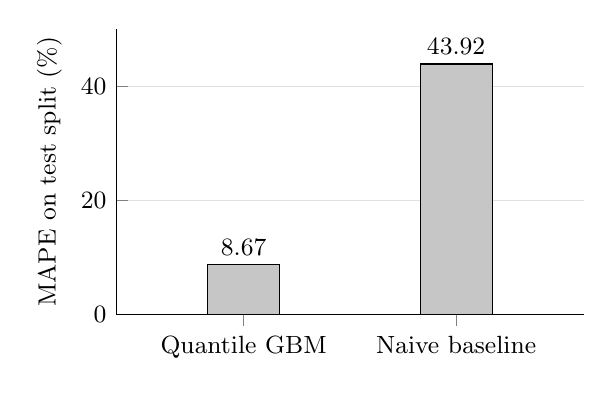
\begin{tikzpicture}
\begin{axis}[
  ybar, width=0.62\textwidth, height=5.2cm, bar width=26pt,
  symbolic x coords={Quantile GBM,Naive baseline}, xtick=data,
  ymin=0, ymax=50, ylabel={MAPE on test split (\%)},
  nodes near coords, nodes near coords align={vertical},
  every node near coord/.append style={font=\small},
  enlarge x limits=0.6, axis lines*=left, ymajorgrids, grid style={gray!25},
  tick label style={font=\small}, label style={font=\small}]
\addplot[fill=gray!45,draw=black] coordinates {(Quantile GBM,8.67) (Naive baseline,43.92)};
\end{axis}
\end{tikzpicture}
\caption{Mean absolute percentage error of the price model and the naive baseline.}\label{fig:mape}
\end{figure}

\section{Analysis}
\begin{itemize}
  \item \textbf{Did we meet our objectives?} Yes. All six objectives of Section~1.2 were implemented:
        verified access, the full buy, borrow, sell and lend workflow, ML-assisted pricing, a consistent
        checkout, trust and privacy, and three independently runnable tiers. Each is exercised by the unit
        and integration tests in Table~\ref{tab:tests}. One metric fell short: the fair band covers
        76.7\,\% of test prices against its 80\,\% target, so it is a useful guide but not a guarantee.
  \item \textbf{Where did we exceed expectations?} The model reduces the percentage error to about one
        fifth of the baseline's (8.67\,\% against 43.92\,\%) and the absolute error to less than half.
        Predictions take about 11\,ms, roughly a tenth of the latency target. Both $R^2$ values are high
        because the original price alone explains most of the variance in rupee terms; this is why MAPE is
        the more informative measure here. Re-running the training script in a different environment
        reproduced the figures closely (MAPE 8.71\,\%, coverage 79.0\,\%).
  \item \textbf{What challenges did we encounter?} Table~\ref{tab:challenges} lists the main problems: no
        backend or database at the start, cross-origin errors, a first price model that generalised poorly,
        wrong original prices typed by sellers, photos bloating the database, and the risk of two buyers
        paying for one item. Testing also showed that throughput fell to about 38 requests per second with
        four parallel clients on two CPUs, so a single worker is enough for a demonstration but not for heavy
        concurrent load.
  \item \textbf{How did we resolve them?} Each challenge was turned into a requirement for the next
        increment, as Table~\ref{tab:challenges} shows. The main caveat remains: all accuracy figures come
        from synthetic data, so they show that the pipeline learns, serves and reports correctly, not how
        accurate it is on real campus prices.
\end{itemize}

\begin{table}[htbp]
\centering
\caption{Main problems met during development and how they were resolved.}\label{tab:challenges}
\small
\begin{tabularx}{\textwidth}{@{}L{5.2cm}X@{}}
\toprule
\textbf{Problem} & \textbf{Resolution}\\
\midrule
The app was a frontend over mock data with no persistence. & Added the Express and Mongoose server, the data
models and REST routes, and connected every page through \code{src/api.js}.\\
MongoDB was not installed on the development machine. & Added an automatic fallback to an in-memory MongoDB
server; the real connection string is a one-line configuration change.\\
Icon components cannot be stored in the database. & Stored an \code{iconKey} string and re-hydrated it to a
component in the client.\\
Cross-origin errors between the Vite and Express ports. & Enabled CORS on the API and proxied \code{/api}
through Vite.\\
An empty database made the interface look broken. & Wrote a seed script and seed automatically when the
collections are empty.\\
The first price model, trained on raw prices, generalised poorly and was hidden by a fixed blend with the
formula. & Predicted the price-to-MRP ratio with monotone quantile models and calibrated bands; passed the
model output through and kept the formula only as a fallback.\\
Sellers typed the rent or a typo into the original-price field. & Recognised the item class and substituted
a typical campus MRP, with lower confidence and a visible note.\\
Photos stored inline in listings bloated the database. & Uploaded photos to Cloudinary with type and size checks,
stored only URLs, and migrated old listings.\\
Two buyers could pay for the same item, and a closed tab could lose a payment. & Added atomic reservations,
signed webhooks, idempotent finalisation and automatic refunds.\\
\bottomrule
\end{tabularx}
\end{table}

% =====================================================================
\chapter{Conclusion}\label{ch:conclusion}

\section{Summary of Work}
Campus Marketplace was designed and implemented as a three-tier system: a React interface, an Express and
MongoDB API, and a FastAPI machine-learning service. All six objectives of Section~1.2 were met. Access is
limited to verified college identities; the platform supports buying, borrowing, selling and lending with a
complete loan life cycle; sellers receive an explainable, calibrated price band with a labelled fallback;
checkout is priced on the server, reserved, verified and refundable; users carry a trust score while exact
locations stay private and photos are validated and stored in the cloud; and the three tiers are
independently runnable and covered by 33 integration tests and 8 unit tests.

\section{Key Findings}
\begin{itemize}
  \item \textbf{Finding 1 -- Choosing the right target matters more than the algorithm.} Predicting a
        scale-free price-to-MRP ratio with monotone constraints reduced the test MAPE to 8.67\,\% against
        43.92\,\% for a naive baseline, and the constraints keep the output sensible where data are thin.
  \item \textbf{Finding 2 -- The server must own every amount and state change.} Reading prices from the
        database, reserving items atomically and finalising payments exactly once removed whole classes of
        errors, and iterative delivery made such problems visible early.
  \item \textbf{Finding 3 -- Unexpected results.} The first Random Forest scored well in validation but
        poorly on the test split, the calibrated band still covered slightly less than its target, and
        concurrent throughput was lower than single-client throughput. Each was found only because results
        were measured and reported honestly.
\end{itemize}

\section{Future Work and Recommendations}
The main limitations of the current system are that the price model is trained on synthetic data, the
Razorpay and Cloudinary integrations have been exercised only in development mode with signed payloads and
stubbed SDK calls, messaging is request-based rather than real-time, and uploaded photos are checked for type
and size but not for content. Recommended next steps are:
\begin{enumerate}
  \item \textbf{Potential enhancements:} real-time chat, push or e-mail reminders for due dates, and
        automated checks on photo content~\cite{sommerville}.
  \item \textbf{Alternative approaches:} retrain the price model on anonymised, consented campus sales
        through the existing export path, and compare it with the current model while monitoring band
        coverage.
  \item \textbf{Scalability improvements:} run several ML service workers and API instances behind a load
        balancer, and move to a managed MongoDB cluster.
  \item \textbf{Integration with other systems:} switch to live Razorpay credentials with dispute handling,
        and connect to the institute's single sign-on.
  \item \textbf{Real-world deployment:} deploy the three tiers with continuous integration and model-drift
        monitoring, and run a usability pilot with a group of students.
\end{enumerate}

\section{Final Remarks}
The project shows that a small team can combine established web engineering practice with lightweight
machine learning to serve a concrete community need. Beyond the working system, it gave practical
experience in requirements analysis, UML modelling~\cite{uml}, REST design, security-conscious
authentication, payment verification, privacy by design, automated testing, and the honest reporting of
model performance.

% =====================================================================
\clearpage
\phantomsection
\addcontentsline{toc}{chapter}{Bibliography}
\renewcommand{\bibname}{Bibliography}
\begin{thebibliography}{Ped+11}
\bibitem[Clo26]{cloudinary} Cloudinary Ltd. \emph{Cloudinary Documentation}.
  \url{https://cloudinary.com/documentation}. Accessed 2026.

\bibitem[Fie00]{fielding} R.~T. Fielding. \emph{Architectural Styles and the Design of Network-based
  Software Architectures}. PhD thesis, University of California, Irvine, 2000.

\bibitem[Fri01]{friedman} J.~H. Friedman. Greedy function approximation: a gradient boosting machine.
  \emph{Annals of Statistics}, 29(5):1189--1232, 2001.

\bibitem[Har12]{oauth} D.~Hardt (ed.). \emph{The OAuth 2.0 Authorization Framework}. RFC 6749, IETF, 2012.

\bibitem[JBS15]{jwt} M.~Jones, J.~Bradley, and N.~Sakimura. \emph{JSON Web Token (JWT)}. RFC 7519, IETF, 2015.

\bibitem[Ke+17]{lightgbm} G.~Ke, Q.~Meng, T.~Finley, T.~Wang, W.~Chen, W.~Ma, Q.~Ye, and T.-Y. Liu.
  LightGBM: A highly efficient gradient boosting decision tree. In \emph{Advances in Neural Information
  Processing Systems 30}, pages 3146--3154, 2017.

\bibitem[KB78]{koenker} R.~Koenker and G.~Bassett. Regression quantiles. \emph{Econometrica},
  46(1):33--50, 1978.

\bibitem[KBC97]{hmac} H.~Krawczyk, M.~Bellare, and R.~Canetti. \emph{HMAC: Keyed-hashing for message
  authentication}. RFC 2104, IETF, 1997.

\bibitem[LB03]{larman} C.~Larman and V.~R. Basili. Iterative and incremental developments: a brief history.
  \emph{IEEE Computer}, 36(6):47--56, 2003.

\bibitem[Met26]{react} Meta Open Source. \emph{React Documentation}. \url{https://react.dev}. Accessed 2026.

\bibitem[Mon26]{mongodb} MongoDB, Inc. \emph{MongoDB Documentation}. \url{https://www.mongodb.com/docs}.
  Accessed 2026.

\bibitem[Nie08]{geohash} G.~Niemeyer. \emph{Geohash}. \url{http://geohash.org}, 2008.

\bibitem[Obj17]{uml} Object Management Group. \emph{Unified Modeling Language (UML), Version 2.5.1}. OMG, 2017.

\bibitem[Ope26]{express} OpenJS Foundation. \emph{Express -- Node.js web application framework}.
  \url{https://expressjs.com}. Accessed 2026.

\bibitem[Ped+11]{sklearn} F.~Pedregosa et~al. Scikit-learn: Machine learning in Python. \emph{Journal of
  Machine Learning Research}, 12:2825--2830, 2011.

\bibitem[Ram26]{fastapi} S.~Ram\'irez. \emph{FastAPI Documentation}. \url{https://fastapi.tiangolo.com}.
  Accessed 2026.

\bibitem[RPC19]{romano} Y.~Romano, E.~Patterson, and E.~J. Cand\`es. Conformalized quantile regression. In
  \emph{Advances in Neural Information Processing Systems 32}, pages 3543--3553, 2019.

\bibitem[Sin84]{sinnott} R.~W. Sinnott. Virtues of the haversine. \emph{Sky and Telescope}, 68(2):159, 1984.

\bibitem[Som16]{sommerville} I.~Sommerville. \emph{Software Engineering}, 10th edition. Pearson, 2016.

\end{thebibliography}

\end{document}
